%%%%%%%%%%%%%%%%%%%%%%%%%%%%%%%%%%%%%%%%%%%%%%%%%%%%%%%%%%%%%%%%%
%
% Project     : Turnverein App
% Title       : 
% File        : architektur.tex Rev. 00
% Date        : 07.07.14
% Author      : Raffael Santschi
%
%%%%%%%%%%%%%%%%%%%%%%%%%%%%%%%%%%%%%%%%%%%%%%%%%%%%%%%%%%%%%%%%%

\chapter{Architektur}\label{chap.architektur}
In diesem Kapitel wird auf die ganze Strukur und die Architektur des Backends und des Apps eingegangen. Die Architektur legt die Grundlage für die Umsetzung und sollte mit Bedacht festgelegt werden.

\section{Übersicht}\label{architektur_uebersicht}
Die Systemumgebung (siehe Abbildung \ref{fig:system_scope}) besteht aus einem Webserver, auf welchem das Backend, die Webseite und neu auch die API-Schnitstelle für das App läuft. Die Web-Schnitstelle für Funktioninäre wird in diesem Bild seperat aufgeführt, da sie viel mehr Funktionen bietet als für normale Mitglieder und Nicht-Mitglieder, sie ist jedoch über die gleiche Webseite ansprechbar. Das RESTful API, mit welcher das App kommuniziert, beherrscht nur die in den Anforderungen benötigten Funktionen.
\begin{figure}[h]
\centering
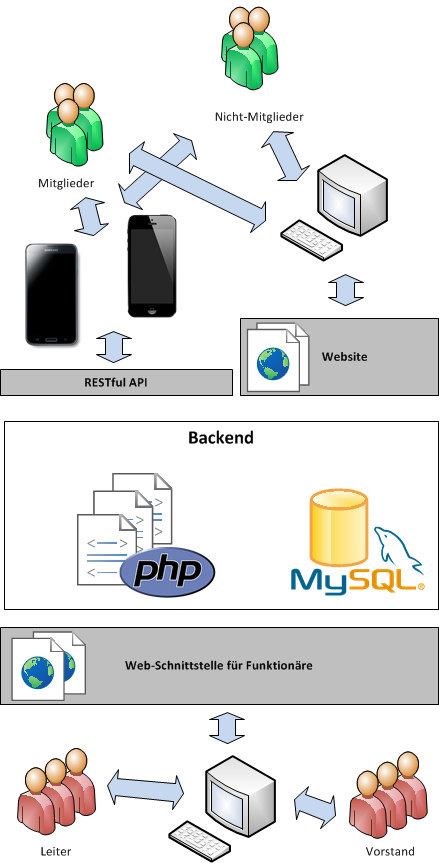
\includegraphics[scale=0.5]{images/visio/SystemScope.png}
\caption{System Übersicht}
\label{fig:system_scope}
\end{figure}

\section{Backend}\label{arch_backend}
Im PHP Backend wird seit diesem Projekt Doctrine (siehe \cite{doctrine} und \cite{dunglas2013persistence}) als Objektrelationaler Mapper (ORM) verwendet. Ein ORM hat den Vorteil, dass man mit einer Konfiguration Tabellen mit Objekten verknüpfen kann und somit viel Arbeit im Bezug auf die Datenbankkommunikation entfällt. Ein Nachteil bei einem ORM kann sein, dass man Funktionen, welche Datenbank spezfisch sind, nicht verwenden kann oder nur mit grossem Aufwand. Doctrine bietet auch Locking-Mechanismen, welche in diesem Projekt benötigt werden. Es gibt die Möglichkeit die Entity-Konfiguration in ein File auszulagern oder mit Annotationen direkt im Objekt zu erfassen, zweiteres ist in diesem Projekt der Fall.

\subsection{Locking}
Das Problem bei einer Fahrgemeinschaftsverwaltung ist, dass man eine beschränkte Anzahl an Plätzen hat. Wenn man beispielsweise davon ausgeht, dass es noch drei freie Plätze hat und vier Mitglieder gleichzeitig auf den Anmelde-Knopf klicken, wäre die Fahrgemeinschaft plötzlich überbucht. Das Szenario ist etwas unwahrscheinlich, die Fahrgemeinschaften werden jedoch immer sehr zeitnah an der Veranstaltung erstellt und somit ist die Zeitspanne, in der sich Mitglieder anmelden, nicht sehr gross. Eine überbuchte Fahrgemeinschaft führt zu Ärger, welcher durch ein gezieltes Locking mit wenig Aufwand vermieden werden kann.\\

Es gibt zwei verschiedene Varianten von Locking, das optimistische Locking und das pessimistische Locking. Das optimistische Locking funktioniert so, dass eine Zeitstempel oder eine Versionsnummer\footnote{Das Verwenden einer Versionsnummer ist die bessere Variante, da ein Zeitstempel bei sehr schnellen und hochfrequenten Transaktionen und je nach Auflösungsgenauigkeit Fehler verursachen könnte.} abgespeichert wird, wenn man das Objekt lädt. Wenn man etwas verändern möchte, wird diese Versionsnummer mitgegeben und geprüft, ob sich die Version seit diesem Zeitpunkt bereits verändert hat. Das pessimistische Locking wird mittels eines Locks, sei es eines zeilenbasierten oder tabellenbasierten Locks, und einer Transaktion umgeben.\\

Die Implementation in diesem Projekt sieht für den User wie ein optimstisches Locking aus, alle vier Mitglieder aus dem Beispiel oben sehen den Anmelde-Knopf, lediglich einer erhält am Schluss die Fehlermeldung, dass es keinen Platz mehr hat. Im Backend ist es jedoch mit einem pessimistischen Locking auf Zeilenebene gelöst. Die Transaktion wird eröffnet, die Zeile wird gelockt, der Request wird überprüft, der Eintrag wird gespeichert und danach wird die Zeile mit dem Beenden der Transaktion wieder freigegeben. Um diesen Vorgang etwas besser zu veranschaulichen wurde ein Sequenzdiagramm (siehe Abbildung \ref{fig:locking_verfahren}) erstellt, dies wurde anhand der Vorlage in \cite{soft_arch_book} realisiert.

\begin{figure}[h]
\centering
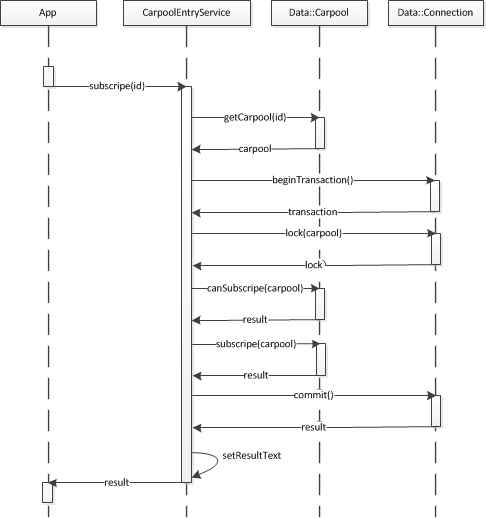
\includegraphics[scale=0.5]{images/visio/locking_verfahren.png}
\caption{Sequenzdiagramm - Locking Verfahren}
\label{fig:locking_verfahren}
\end{figure}

\FloatBarrier
\subsection{API}
Das App hält so gut wie keine Daten vor, sondern holt diese immer direkt vom Backend. Dazu wurde ein RESTful API erstellt, welches JavaScript Object Notation-Objekte (JSON-Objekte) zurück liefert. Das API funktioniert nach dem De-facto-Standard (siehe \cite{wiki_restful}). Bei einem Listen-Aufruf ohne Einträge liefert es eine leere Liste zurück, wenn ein spezifisches Objekt abgerufen wird, liefert es 'null' zurück. Bei Aktionen wird ein JSON-Objekt mit den Attributen 'success' und 'error\_message' zurück gegeben.\\

Das API hat eine Versionsnummer in der URL, damit kann sichergestellt werden, dass ältere Versionen von der App immer noch lauffähig sind, wenn etwas an der Schnittstelle geändert wird. Dieser Punkt ist sehr wichtig, da man den Usern nicht vorschreiben kann, wann und ob sie ihr App updaten.

\section{Lösungsvarianten}\label{loesungsvarianten}
Es gibt verschiedene Wege ein App zu entwickeln und jede hat seine Vor- und Nachteile. In diesem Abschnitt werden drei verschiedenen Methoden miteinander verglichen und die beste für diesen Anwendungszweck ausgewählt.

\subsection{Native App}\label{architektur_native}
Früher gab es nur diese Variante der App Entwicklung, man musste für jede Plattform die bereitgestellte Integrated Development Environment (IDE) verwenden und die dazugehörige Sprache lernen. Bei Apple ist das XCode und Objective-C, bei Android früher Eclipse Android Development Tools (ADT) und heute Android Studio basierend auf IntelliJ beide Male mit der Programmiersprache Java. Die Vorteile sind voller Funktionsumfang und gute Unterstützung bei der Entwicklung durch die IDE's. Das führen von zwei oder mehreren seperaten Code-Sourcen ist jedoch sehr aufwendig und mühsam.

\subsection{Xamarin}\label{architektur_xamarin}
Xamarin (siehe \cite{xamarin}) ist ein sehr mächtiges Framework, welches ermöglicht den Code der App in C\# zu schreiben und diesen dann in Native Code umzuwandeln. Xamarin liefert seine eigene IDE kann aber auch in Visual Studio integriert werden. Grosse Firmen wie 3M, AT\&T und HP verwenden Xamarin für ihre Apps. Der grosse Vorteil ist, dass man fast alle Funktionen einer Native App verwenden kann und dazu nur eine Sprache und eine IDE beherrschen muss.

\subsection{Phonegap}\label{architektur_phonegapt}
Phonegap (siehe \cite{phonegap} und \cite{wargo2012phonegap}) basiert auf Cordova (siehe \cite{cordova}), ein Framework von Apache, mit welchem es möglich ist, eine Webseite geschrieben in HTML und Javascript in eine Native App umzuwandeln. Phonegap bietet Javascript Plugins um die Native Funktionen wie zum Beispiel Geolocation, Kompass oder Push-Nachrichten zu benutzen. Das Framework erstellt für die gewünschte Plattform ein App mit einer Webview und fügt die nötigen Klassen für die Plugins hinzu. Ein positiver Nebeneffekt ist bei dieser Methode, dass man die Webseite auch online stellen kann und alles ausser die Plugins benutzt werden kann. Phonegap bietet im Gegensatz zu den anderen Varianten keine Unterstützung zum Modellieren oder Erstellen grafischer Benutzeroberflächen. Es kümmert sich lediglich um die Konvertierung in die verschiedenen Plattformen und stellt die Schnittstellen zu den Native Funktionen bereit. Phonegap wird oft mit einem für mobile Geräte optimiertem Framework wie zum Beispiel jQuery Mobile (siehe \cite{jquery_mobile} und \cite{reid2011jquery}) kombiniert.

\newpage
\subsection{Nutzwertanalyse}\label{architektur_nutzwertanalyse}

\subsubsection{Bewertungskriterien}\label{architektur_bewertungspunkte}

In der Nutzwertanalyse werden folgende Punkte betrachtet und nach dem angegebenen Schema bewertet und anschliessend gewichtet. Die Kriterien sind grösstenteils aus den Softwarequalitäsmerkmalen nach \cite{iso_9126} abgeleitet.

\paragraph{Aufwand}
\begin{itemize}
	\item \textbf{Beschreibung}: Wie gross ist der geschätzte Aufwand mit dieser Methode?
	\item \textbf{Bewertung}: 1: sehr hoch, 10: sehr niedrig
	\item \textbf{Gewichtung}: 5 (Die Zeit für dieses Projekt ist beschränkt und die Entscheidung könnte zu einem Risiko werden)
\end{itemize}

\paragraph{Benutzbarkeit}
\begin{itemize}
	\item \textbf{Beschreibung}: Wie schnell hat man diese Variante erlernt? 
	\item \textbf{Bewertung}: 1: sehr langsam, 10: sehr schnell
	\item \textbf{Gewichtung}: 4 (Umso mehr Zeit für das Erlernen investiert wird, umso weniger Zeit hat man für die Implementierung)
\end{itemize}

\paragraph{Übertragbarkeit}
\begin{itemize}
	\item \textbf{Beschreibung}: Wie flexibel ist diese Variante? Kann sie auf verschiedenen Plattformen laufen? 
	\item \textbf{Bewertung}: 1: sehr spezifisch, nicht portabel, 10: sehr flexibel
	\item \textbf{Gewichtung}: 4 (Die Anforderungen geben vor, dass das App mindestens auf Android und iOS laufen muss)
\end{itemize}

\paragraph{Funktionalität}
\begin{itemize}
	\item \textbf{Beschreibung}: Wie gross ist der Funktionalitätsumfang? 
	\item \textbf{Bewertung}: 1: sehr eingeschränkt, 10: sehr weit reichend
	\item \textbf{Gewichtung}: 3 (In der ersten Version der App wird noch nicht viel Funktionalität gebraucht)
\end{itemize}

\paragraph{Kosten}
\begin{itemize}
	\item \textbf{Beschreibung}: Wie viel kostet diese Lösung? 
	\item \textbf{Bewertung}: 1: sehr teuer, 10: gratis
	\item \textbf{Gewichtung}: 1 (Der Turnverein kommt für die Kosten auf und ist auch bereit etwas dafür zu bezahlen)
\end{itemize}

\newpage
\subsubsection{Bewertung}\label{architektur_bewertung}
Anhand der zuvor definierten Kriterien wurde eine Bewertung vorgenommen. Diese Bewertung ist nicht generell gültig, sie bezieht sich auf die Erfahrung des Entwicklers dieser Arbeit und das Projekt selbst.

\begin{table}[ht]
\centering
  \begin{tabular}{>{\columncolor{darkgray}} l | p{4cm} | p{4cm} | p{4cm}}
	\hline
	\rowcolor{darkgray}
	Kriterium		&	Native App	&	Xamarin 	&	Phonegap	\\ \hline
				&	
\includegraphics{images/icons/ios_android.png}	&	
\includegraphics[scale=0.25]{images/icons/xamarin.png} 	&	
\includegraphics[scale=0.25]{images/icons/phonegap_logo.jpg}	\\ \hline
	\rowcolor{gray}
	Aufwand		&	2 (10)		&	4 (20)		&	7 (35)		\\ \hline
	Begründung		&	Schon beim Support von 2 Plattformen enorm gross	
				&	C\# lernen, in Xamarin einarbeiten			
				&	jQuery Mobile erlernen, Phonegap kennen lernen	\\ \hline
	\rowcolor{gray}
	Benutzbarkeit	&	5 (20)		&	4 (16)		&	7 (28)		\\ \hline
	Begründung		&	Die IDEs sind sehr umgänglich, jedoch nicht sehr viel Erfahrung in Objectiv-C
				&	Keine Erfahrung in C\# und fast keine Erfahrung mit Visual Studio/Xamarin				
				&	Viel Erfahrung in HTML/Javascript, jedoch keine Erfahrung mit jQuery Mobile\\ \hline
	\rowcolor{gray}
	Übertragbarkeit	&	2 (8)		&	7 (28)		&	8 (32)		\\ \hline
	Begründung		&	Jede Plattform seinen eigenen Code	
				&	Einschränkung bei der Wiederverwendung von UI Code				
				&	Ausser einigen Zeilen exakt der gleiche Code	\\ \hline
	\rowcolor{gray}
	Funktionalität	&	10 (30)	&	9 (27)		&	7 (21)		\\ \hline
	Begründung		&	Alles was die Produkte bietet, kann verwendet werden		
				&	Nahezu alles kann verwendet und gemacht werden				
				&	Plugins bieten nicht den kompletten Funktionsumfang	\\ \hline
	\rowcolor{gray}
	Kosten		&	9 (9)		&	3 (3)		&	9 (9)		\\ \hline
	Begründung		&	Developer Accounts kosten, ansonsten gratis		
				&	Developer Accounts kosten, jedoch Kosten pro Plattform				
				&	Developer Accounts kosten, ansonsten gratis		\\ \hline \hline
	\rowcolor{gray}
	\textbf{Total (gewichtet)}	&	\textbf{28 (77)}	&	\textbf{27 (94)}	&	\textbf{38 (125)}	\\ \hline
  \end{tabular}
   \caption{Nutzwertanalyse - App Variante}\label{table:bewertungskriterien}
\end{table}

\FloatBarrier
\subsubsection{Fazit}\label{architektur_fazit}
Das Resultat der Nutzweranalyse ist eindeutig, die Entwicklung mittels Phonegap ist für dieses Projekt mit Abstand die beste Lösung. Die Methode hat noch weitere Vorteile: Etwa dass der Code nur in eine App verpackt wird und er nicht in eine andere Sprache übersetzt werden muss -- somit gibt es viel weniger Overhead. Zudem ist es möglich den Quellecode in der App anzupassen, dass heisst, falls der Converter nicht mehr funktioniert, weil er zum Beispiel nicht mehr unterhalten wird, kann man trotzdem noch weiterentwickeln und muss nicht zuerst ein Reverse Engineering machen.

\newpage
\section{Mobile App}\label{moblie_app}

Die Nuzwertanalyse \ref{architektur_nutzwertanalyse} hat gezeigt, dass die beste Methode für dieses Projekt das Phonegap Framework ist. Dies wurde im Projekt auch so umgesetzt und mit jQuery Mobile kombiniert. jQuery Mobile hat die Grundidee, alle Seiten im selben HTML-File zu speichern, bietet jedoch auch die Möglichkeit, die Seiten in verschiedene Files aufzuteilen. In diesem Projek wurde die zweite Variante gewählt, weil damit zwar ein wenig Code-Duplikation generiert wurde, aber jede Seite einzel getest werden konnte, nur die nötigen Elemente geladen werden müssen und vorallem damit die HTML-Files übersichtlich bleiben. Die einzelnen Seiten sind sehr einfach aufgebaut, sie bestehen aus einem Header, in welchem das Menü, bzw. in Unterseiten die Back-Taste, und die Einstellungen aufgerufen werden können. Der Inhalt wird in einer ListView angezeigt. Die Daten werden über einen jeweiligen Asynchronous JavaScript and XML-Request (Ajax-Request) vom Backen abgeholt und dann in die ListView abgefüllt.\\

Von Phonegap wurden die Plugins PushNotification, für das Empfangen von Push-Nachrichten, und Device verwendet. Das PushNotification Plugin muss für Android und iOS spezifisch initialisiert werden und um herauszufinden, auf welcher Plattform das App läuft, wurde das Device Plugin verwendet. \\



